\setcounter{figure}{0}

\section{9th July 2023: God's love for us and our holiness}
\subsection*{Text: 1 John 2:28-3:3}
  \begin{quote}
    [28] And now, little children, abide in him, so that when he appears we may have confidence and not shrink from him in shame at his coming. [29] If you know that he is righteous, you may be sure that everyone who practices righteousness has been born of him.

    [1] See what kind of love the Father has given to us, that we should be called children of God; and so we are. The reason why the world does not know us is that it did not know him. [2] Beloved, we are God’s children now, and what we will be has not yet appeared; but we know that when he appears we shall be like him, because we shall see him as he is. [3] And everyone who thus hopes in him purifies himself as he is pure.
  \end{quote}
\subsection*{Notes}
\begin{itemize}
  \item{Our privileged status as God’s people is based on two things: God’s unconditional love and God’s promises.}
  \item{ For the first point on God’s unconditional love, it is even true in
  the OT, i.e Deuteronomy 7:7. This point directly addresses the spirit of
  entitlement in our culture. And this spirit of entitlement has crept into
  the church! Sometimes, we might think: “Lord, pls help me with X, then I
  will do Y”. We feel entitled to God to do certain things for us. But rather
  than asking God to conform to our will, we should conform our wills to
  God’s will, in response to God’s unconditional love for us. We don’t need
  to do things for God to love us. God loves us even while we were still
  sinners. Its just that God’s love is more mysterious than we can ever
  understand, so we must just trust. Rather than have a spirit of
  entitlement. }
  \item{For the second point on God’s promises, we know that God will not go
  back on His word. God has promised us many things, such as His presence,
  His salvation, etc. In our text, God has promised that we will not shrink
  from Jesus in shame when He comes again, but this promise is a conditional
  promise; the condition is that we must abide in Jesus. And abiding in Jesus
  necessarily means forsaking sin and forsaking the acceptance/sinful
  pleasures of the world, and then walking in the way of the Lord. }
  \item{ When we forsake the world, the world will hate us, as Jesus
  mentioned in the sermon on the mount. But when we are being attacked, we
  can identify with Christ in His suffering, and it also shapes us to be more
  Christlike.}
  \item{In 1 John 3, we see that our hope is to be like Jesus as He is,
  and see Jesus as who He really is. Since that is our hope, we are to strive
  to resemble Jesus in holiness now, so we can have some measure of that! And
  when we resemble Jesus in holiness now, we testify to the world that we
  belong to God, c.f 1 Peter 2:9 and Deuteronomy 7:6. }
  \item{God’s saving grace is always accompanied by His transforming grace! We don’t strive to be holy to be saved, but instead we strive to be holy because we are saved. Holiness is not just the outward forms of piety like going to church. Holiness is a state of mind stemming from our real relationship with God.}
  \item{Application: we need self examination to see if we are truly born again and saved. Since a holy life and a pure life that strives to fight sin daily and to hate sin is a necessary (but not sufficient condition) for salvation, we need to check if we have compromised with sin in any way. The sufficient condition for salvation is for us to trust Jesus, and for that we need to check if we have a relationship of trust in Jesus and Jesus alone. Do we trust Jesus for our justification? Do we trust Jesus for His power to sanctify us? Do we trust Jesus to provide for our needs, both physical and spiritual? How is our trust manifested in practical actions?
  \begin{itemize}
    \item{Tl;dr: do we hate sin? (Necessary but not sufficient condition for salvation). Do we trust Jesus and in Jesus alone, for our physical and more importantly our spiritual needs? (sufficient condition for salvation)}
  \end{itemize} }
  % \item{\begin{figure}[H]
  %   \centering
  %   % 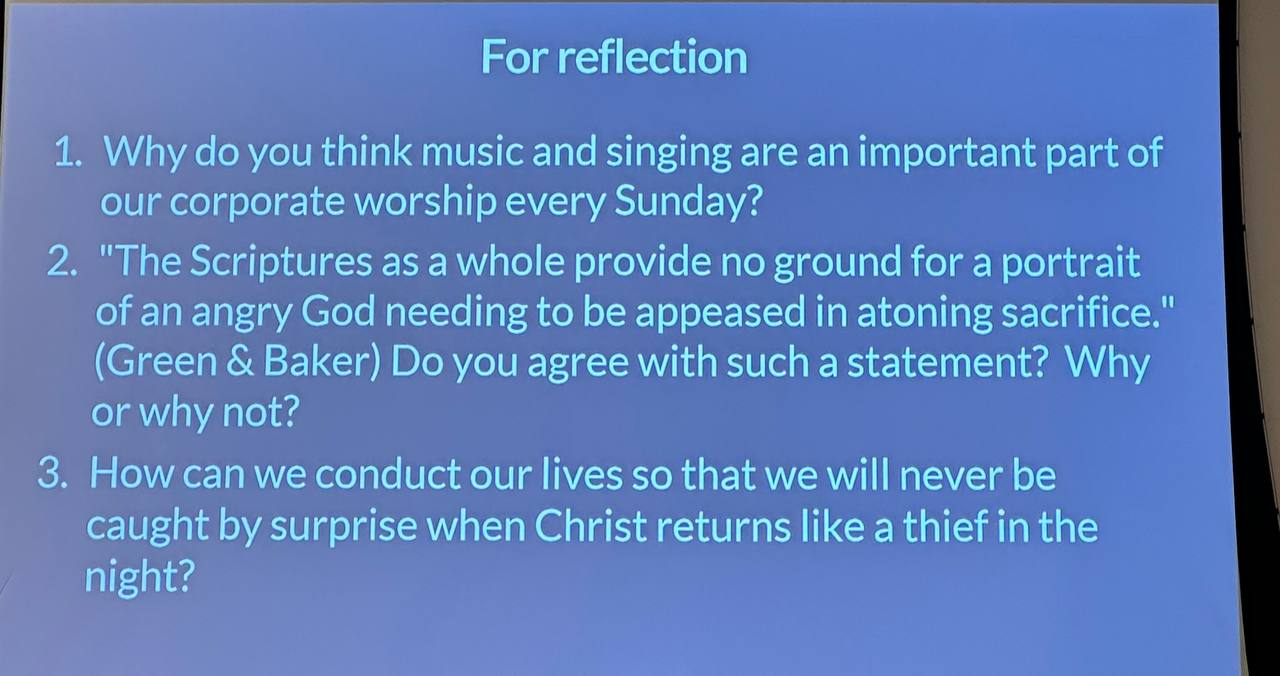
\includegraphics[width=0.8\textwidth, trim={0cm 0cm 0cm 0cm},clip]{Figures/marchSermon4Reflections.jpg}
  %   \includegraphics[width=0.8\textwidth, trim={0cm 0cm 0cm 0cm},clip]{example-image-a}
  %   \caption[]{Reflection questions for this sermon}
  %   \label{}
  % \end{figure}}
\end{itemize}